\documentclass[11pt,a4paper]{article}
\usepackage[T1]{fontenc}
\usepackage[margin=2.3cm]{geometry}
\usepackage{amsmath,amssymb}
\usepackage{graphicx}
\usepackage[dvipsnames]{xcolor}
\usepackage{enumitem}
\usepackage[colorlinks=true,linkcolor=blue,urlcolor=blue]{hyperref}
\setlength{\parskip}{0.6em}
\setlength{\parindent}{0pt}
\begin{document}

\begin{center}{\LARGE\bfseries openfloat}\\[0.4em]{\large Learn why computers get arithmetic wrong, from 0.1 + 0.2 to the Patriot and Ariane 5 failures.}\\[0.2em]\small PAN IIT OSS explainer \textbullet{} secondary school to diploma / undergraduate (levels 3-5)\end{center}

\section*{Why this exists}
Every computer stores real numbers with a limited number of binary digits. This explainer shows how that creates gaps between numbers, how rounding errors appear and pile up, and how two real failures can be traced to number-format limits, using only simple arithmetic.

\section*{The end goal}
Learn from floating-point disasters like Patriot and Ariane 5. The end goal is to learn from floating-point disasters such as Patriot and Ariane 5: to recognise where precision and range are lost and to design calculations that stay safe. The same habits matter in simulation, finance, graphics and control.

\section*{How the three sessions build up}
\begin{enumerate}[nosep]
\item \textbf{Session 1: Numbers with gaps} (Level 1, conceptual interactive model, 60 min).
\item \textbf{Session 2: The 64-bit format, rounding and cancellation} (Level 2, mathematical engineering model, 75 min).
\item \textbf{Session 3: Accumulated error: Patriot, Ariane 5 and safe summation} (Level 3, simulation and validation, 90 min).
\end{enumerate}

\section{Session 1: Numbers with gaps}

\subsection*{A. Real-world problem}
Type 0.1 + 0.2 into almost any programming language. The answer is 0.30000000000000004, and 0.1 + 0.2 == 0.3 is False. A spreadsheet, a phone calculator and a flight computer all store numbers using a limited number of binary digits. Between two storable numbers there is a gap, and every result has to be rounded to a storable number. How big are the gaps, where are they large, and how do we program safely around them?

\subsection*{B. Concept and theory}
Computers write numbers in binary. A decimal fraction such as 0.1 becomes the repeating binary pattern 0.000110011..., which never ends, just as 1/3 = 0.333... never ends in decimal. A computer keeps only a fixed number m of binary digits after the leading 1 (the fraction bits), so it can store only certain numbers. Between 2\textasciicircum{}k and 2\textasciicircum{}(k+1) the stored numbers are equally spaced, 2\textasciicircum{}m of them, with gap 2\textasciicircum{}(k-m). When x doubles, the gap doubles. So the gap is small near 0 and large for big numbers, but the relative gap (gap divided by x) stays between 2\textasciicircum{}-m / 2 and 2\textasciicircum{}-m. The 64-bit format used by Python and NumPy has m = 52. A result that falls between two stored numbers is rounded to a nearby stored one, which is the source of every effect in this repo. Instead of testing a == b for computed numbers, test whether they differ by less than a tolerance chosen relative to their size.

\begin{itemize}[nosep]
\item m: number of fraction bits (52 for 64-bit floats) (no unit)
\item k: exponent: x lies in [2\textasciicircum{}k, 2\textasciicircum{}(k+1)) (no unit)
\item gap: distance from x to the next stored number (same unit as x)
\item relative gap: gap divided by x (no unit)
\end{itemize}

\begin{equation*}
\mathrm{gap}(x)=2^{k-m},\qquad 2^k\le x<2^{k+1}
\end{equation*}

\begin{equation*}
\frac{2^{-m}}{2}<\frac{\mathrm{gap}(x)}{x}\le 2^{-m}
\end{equation*}

\begin{equation*}
\varepsilon_{\mathrm{mach}}=\mathrm{gap}(1)=2^{-52}\approx 2.22\times10^{-16}\quad(m=52)
\end{equation*}

\begin{center}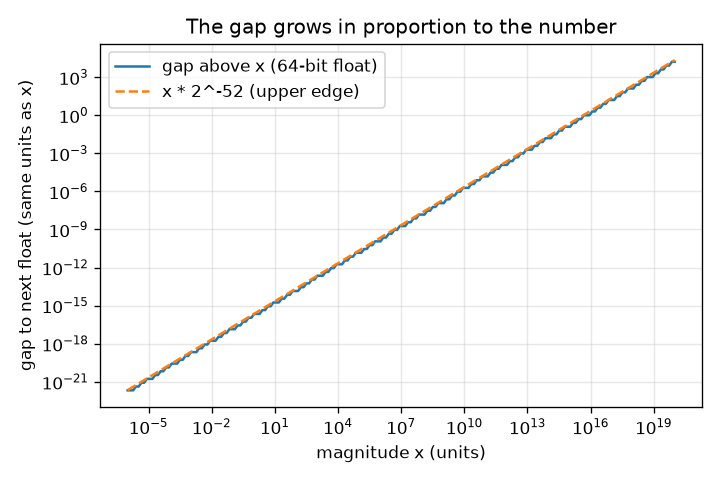
\includegraphics[width=0.85\linewidth]{figures/s01_gap_vs_magnitude.png}\\\small The real 64-bit gap grows in proportion to the number (log-log axes).\end{center}

\subsection*{E. Worked example}
Find the gap above 1000 in the 64-bit format by hand, then check it by computer. Also explain why 2\textasciicircum{}53 + 1 equals 2\textasciicircum{}53.
\begin{enumerate}[nosep]
\item 1000 lies between 512 = 2\textasciicircum{}9 and 1024 = 2\textasciicircum{}10, so k = 9.
\item gap = 2\textasciicircum{}(k - 52) = 2\textasciicircum{}(9 - 52) = 2\textasciicircum{}-43.
\item 2\textasciicircum{}-43 = 1.137e-13. The relative gap is 1.137e-13 / 1000 = 1.137e-16, between 1.1e-16 and 2.2e-16 as predicted.
\item For 2\textasciicircum{}53: k = 53, so gap = 2\textasciicircum{}(53 - 52) = 2. The next number after 2\textasciicircum{}53 is 2\textasciicircum{}53 + 2, so 2\textasciicircum{}53 + 1 falls halfway and is rounded back to 2\textasciicircum{}53.
\end{enumerate}
\textbf{Answer.} The gap above 1000 is 2\textasciicircum{}-43, about 1.137e-13 (relative 1.137e-16). Above 2\textasciicircum{}53 (about 9.0e15) the gap is 2, so whole numbers can no longer all be stored.

\subsection*{F. Questions}
\begin{enumerate}[nosep]
\item \textbf{Conceptual.} Why can 0.5 be stored exactly but 0.1 cannot?
\item \textbf{Numerical.} What is the gap just above 1000.0 in a 64-bit float? What is the relative gap? Does your answer pass a sanity check?
\item \textbf{Graph and simulation interpretation.} In the graph view with 3 fraction bits, what is the gap for numbers in [8, 16) and how many numbers are stored there? What changes if you use 5 fraction bits?
\item \textbf{Design and optimisation challenge.} Design: a toy sensor must store lengths from 1 to 16 units with a gap of at most 0.1 units everywhere. How many fraction bits m are needed? What is the cost of using more?
\end{enumerate}

\section{Session 2: The 64-bit format, rounding and cancellation}

\subsection*{A. Real-world problem}
An engineer solves x\textasciicircum{}2 - 1,000,000 x + 1 = 0 with the textbook formula and finds the small root is 1.0000076e-6; the true value is 1.000000000001e-6. A physicist computes 1 - cos(0.00000001) and gets exactly 0. Both used correct formulas on a correct computer. What went wrong, how many digits did we lose, and what is the rule that tells us which formulas to avoid? And what happens if a number is simply too large or too small for the format?

\subsection*{B. Concept and theory}
A normal 64-bit number is stored in 64 bits: 1 sign bit s, 11 exponent bits e (a whole number from 1 to 2046) and 52 fraction bits f. Its value is (-1)\textasciicircum{}s (1 + f / 2\textasciicircum{}52) 2\textasciicircum{}(e - 1023). The leading 1 is implied. Machine epsilon 2\textasciicircum{}-52 (about 2.22e-16) is the gap above 1. Rounding to the nearest stored number makes a relative error of at most u = 2\textasciicircum{}-53 (about 1.1e-16): fl(x) = x (1 + delta) with \textbar{}delta\textbar{} \textless{}= u. A single operation is therefore accurate to about 16 digits. Subtracting two nearly equal numbers is the dangerous operation: the leading digits cancel exactly, and what remains is dominated by the old rounding errors, so the relative error of the difference can be huge (catastrophic cancellation). The remedy is algebra: rewrite the formula so that it adds like-signed terms. For x\textasciicircum{}2 - b x + c = 0 with b \textgreater{} 0 large, the small root (b - sqrt(b\textasciicircum{}2 - 4c))/2 subtracts two nearly equal numbers; compute the large root (b + sqrt(b\textasciicircum{}2 - 4c))/2 first and then use x1 x2 = c to get x2 = c / x1. For small angles, 1 - cos(t) = 2 sin\textasciicircum{}2(t / 2) avoids the subtraction. The range of a 64-bit float is about 2.2e-308 (smallest normal) to 1.8e308 (largest). Larger results become inf (overflow); smaller ones lose digits as subnormal numbers (down to 5e-324) and then become 0 (underflow). sqrt(x\textasciicircum{}2 + y\textasciicircum{}2) overflows for x = 3e200 even though the answer, 5e200, is representable; scale first.

\begin{itemize}[nosep]
\item s, e, f: sign bit, exponent field (11 bits), fraction field (52 bits) (no unit)
\item u: unit round-off 2\textasciicircum{}-53, about 1.1e-16 (no unit)
\item eps: machine epsilon 2\textasciicircum{}-52, about 2.22e-16 (no unit)
\item b, c: coefficients of x\textasciicircum{}2 - b x + c = 0 (no unit)
\item x1, x2: large and small root (no unit)
\item t: angle (radians)
\end{itemize}

\begin{equation*}
x=(-1)^s\left(1+\frac{f}{2^{52}}\right)2^{\,e-1023}
\end{equation*}

\begin{equation*}
\mathrm{fl}(x)=x(1+\delta),\quad |\delta|\le u=2^{-53}\approx1.1\times10^{-16}
\end{equation*}

\begin{equation*}
x_1=\frac{b+\sqrt{b^2-4c}}{2},\qquad x_2=\frac{c}{x_1}\qquad\text{(instead of }x_2=\tfrac{b-\sqrt{b^2-4c}}{2}\text{)}
\end{equation*}

\begin{equation*}
1-\cos t=2\sin^2\!\left(\frac t2\right)
\end{equation*}

\begin{equation*}
\text{relative error of the textbook small root}\ \lesssim\ u\,b^2/c\quad(b^2\gg 4c)
\end{equation*}

\begin{center}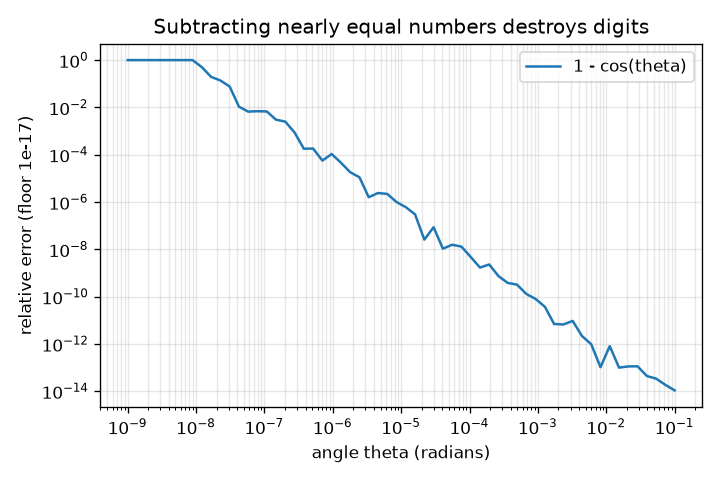
\includegraphics[width=0.85\linewidth]{figures/s02_one_minus_cos_error.png}\\\small Error of 1 - cos(t) for small angles t: digits are destroyed by the subtraction.\end{center}

\subsection*{E. Worked example}
(a) Decode -6.5 into sign, exponent field and fraction field. (b) For x\textasciicircum{}2 - 1e6 x + 1 = 0, compute the small root with both formulas and measure the error. (c) Show why 1 - cos(1e-8) is exactly 0.
\begin{enumerate}[nosep]
\item (a) -6.5 = -1.625 x 2\textasciicircum{}2. Sign bit s = 1. True exponent 2, so e = 2 + 1023 = 1025. Fraction: 1.625 = 1 + 0.625, so f = 0.625 x 2\textasciicircum{}52 (hexadecimal a000000000000).
\item (b) b = 1e6, c = 1. sqrt(b\textasciicircum{}2 - 4) = 999999.999998, very close to b = 1e6. The textbook small root (b - sqrt(...))/2 subtracts two numbers equal in their first 12 digits and gives 1.00000761449e-6. The stable route gives x1 = 1e6 (to 16 digits) and x2 = 1 / x1 = 1.000000000001e-6, which agrees with 60-digit arithmetic.
\item Relative error of the textbook root = 7.6e-6, so only about 5 correct digits remain (11 digits lost). The estimate u b\textasciicircum{}2 / c = 1.1e-4 is an upper-bound estimate and the measured error is below it.
\item (c) For t = 1e-8, cos t = 1 - t\textasciicircum{}2/2 = 1 - 5e-17. The gap just below 1 is 2\textasciicircum{}-53 = 1.1e-16, so 1 - 5e-17 is closer to 1 than to the next number below it (distance 5e-17 against 6e-17). cos(1e-8) is stored as 1.0 and 1 - cos = 0. The stable formula gives 2 sin\textasciicircum{}2(5e-9) = 5.0e-17.
\end{enumerate}
\textbf{Answer.} -6.5: s = 1, e = 1025, f = 0.625 x 2\textasciicircum{}52. The textbook small root of x\textasciicircum{}2 - 1e6 x + 1 has relative error 7.6e-6 (about 5 correct digits); the stable formula is correct to about 16. 1 - cos(1e-8) computes to 0 although the true value is 5e-17.

\subsection*{F. Questions}
\begin{enumerate}[nosep]
\item \textbf{Conceptual.} Why does computing 1 - cos(1e-8) give exactly 0 although each single operation is accurate to 16 digits?
\item \textbf{Numerical.} Decode 0.15625 (that is 5/32): give s, e and the fraction field f. Sanity check by rebuilding the value.
\item \textbf{Graph and simulation interpretation.} From the app graph view (c = 1), roughly how does the error of the textbook small root change when p increases by 1? About how many digits are correct at p = 6?
\item \textbf{Design and optimisation challenge.} Design: a program must evaluate 1 - cos(t) for every angle from 1e-9 to 1 radian with a relative error below 1e-12. Choose the formula(s). Where, if anywhere, is the textbook form acceptable?
\end{enumerate}

\section{Session 3: Accumulated error: Patriot, Ariane 5 and safe summation}

\subsection*{A. Real-world problem}
Two famous failures need no exotic mathematics. In February 1991 a Patriot air-defence battery in Dhahran had been running for about 100 hours; its clock counted time in tenths of a second, and 0.1 cannot be stored exactly in binary. The commonly cited analysis says the tiny error added at every tick had grown to about a third of a second, enough to shift where the system looked for an incoming Scud. In June 1996 the first Ariane 5 flight was lost when software raised an exception after an unprotected conversion of a 64-bit floating-point value to a 16-bit signed integer. Can we reproduce the mechanisms with a few lines of code, and learn the defences? This is a simplified educational model, not an account of either system; read the official reports for the full stories.

\subsection*{B. Concept and theory}
Naive (recursive) summation adds one term at a time, and every addition rounds, adding an error of up to u times the partial sum. The standard worst-case bound for n terms is (n - 1) u times the sum of the absolute values; the error can grow in proportion to n, and the measured error is often smaller. Kahan summation carries a correction c: for each x, y = x - c; t = s + y; c = (t - s) - y; s = t. It captures the part of y lost in the addition and subtracts it next time; its error bound is about 2u times the sum of absolute values, independent of n, plus a term of order n u\textasciicircum{}2. math.fsum keeps exact partial sums and rounds once. For the Patriot calculation, time was counted in ticks of 0.1 s. With 0.1 chopped (not rounded) to q binary places the stored tick is 0.1 - delta where delta is the chopped-off remainder; with the commonly cited 24-bit register holding 23 places after the point, delta = 0.1 x 2\textasciicircum{}-20, about 9.5e-8 s. After h hours there are 36000 h ticks, so the clock is late by 36000 h delta, a straight line in time. At 100 hours that is 0.343 s, and at the commonly cited Scud speed of about 1676 m/s the target moves about 575 m, more than half a kilometre, in that time. For the integer conversion: a 16-bit signed integer holds -32768 to 32767. An unchecked conversion of a larger value can wrap around modulo 65536 (for example 40000 becomes -25536) or, in some languages, raise an exception. The defence is to check the range first and then choose: raise, saturate, or report.

\begin{itemize}[nosep]
\item n: number of terms in a sum (no unit)
\item u: unit round-off 2\textasciicircum{}-53 (no unit)
\item q: binary places kept after the point (23 in the commonly cited Patriot layout) (no unit)
\item delta: error per 0.1 s tick after chopping (s)
\item h: hours of operation (h)
\item v: speed of the target (about 1676 m/s, commonly cited) (m/s)
\end{itemize}

\begin{equation*}
|E_n|\le (n-1)\,u\sum_{i=1}^{n}|x_i|\qquad\text{(recursive summation, worst case)}
\end{equation*}

\begin{equation*}
y=x-c,\quad t=s+y,\quad c=(t-s)-y,\quad s=t\qquad\text{(Kahan)}
\end{equation*}

\begin{equation*}
\delta=0.1-\frac{\lfloor 0.1\cdot 2^{q}\rfloor}{2^{q}},\qquad \delta(q{=}23)=0.1\cdot 2^{-20}\approx 9.54\times10^{-8}\ \mathrm{s}
\end{equation*}

\begin{equation*}
\text{clock error}=36000\,h\,\delta,\qquad \text{distance}=v\times\text{clock error}
\end{equation*}

\begin{equation*}
\text{wrap}(x)=\big((x+32768)\bmod 65536\big)-32768
\end{equation*}

\begin{center}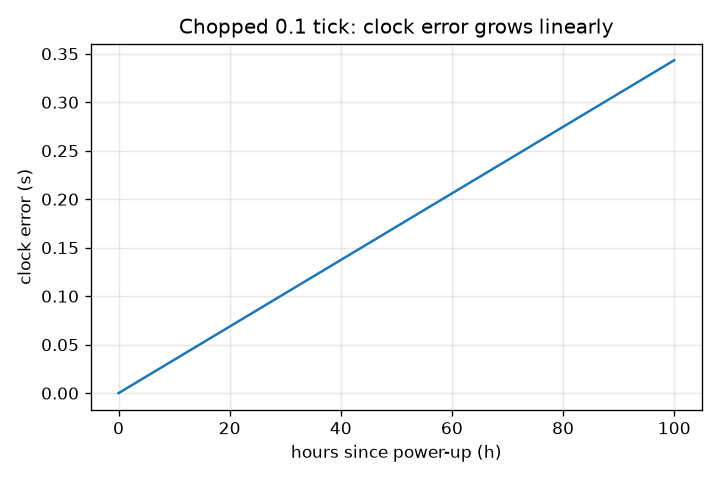
\includegraphics[width=0.85\linewidth]{figures/s03_patriot_drift.png}\\\small Clock error against hours for 0.1 chopped to 23 binary places: a straight line, 0.343 s at 100 hours.\end{center}

\subsection*{E. Worked example}
(a) Compute the Patriot clock error after 100 hours and the distance a 1676 m/s target covers in that time, from 0.1 chopped to 23 places. (b) What does 40000 become in a 16-bit signed integer? (c) State the measured error of summing 0.1 ten million times, naive versus Kahan.
\begin{enumerate}[nosep]
\item (a) 0.1 = 0.0001100110011... in binary. Chopping at 23 places leaves a remainder of 0.1 x 2\textasciicircum{}-20 = 9.54e-8 s per tick (checked in the lesson with exact fractions).
\item 100 hours = 100 x 3600 s = 360000 s = 3,600,000 ticks. Clock error = 3,600,000 x 9.5367e-8 = 0.3433 s.
\item Distance = 1676 m/s x 0.3433 s = 575 m, about 0.58 km, in line with the commonly cited 'about half a kilometre'.
\item (b) 40000 is above 32767. Wrap: (40000 + 32768) mod 65536 - 32768. First 72768 mod 65536 = 7232, then 7232 - 32768 = -25536. A value of 40000 becomes -25536.
\item (c) Ten million terms: the exact reference is 1,000,000 (rounded to a 64-bit float). The naive sum is off by 1.6e-4, below the worst-case bound 1.1e-3 (about 7 times lower). Kahan and math.fsum are off by 0.0.
\end{enumerate}
\textbf{Answer.} Clock error 0.343 s after 100 hours; the target moves about 575 m. 40000 wraps to -25536. Summing 0.1 ten million times naively is off by about 1.6e-4; Kahan and fsum give the correctly rounded 1,000,000.

\subsection*{F. Questions}
\begin{enumerate}[nosep]
\item \textbf{Conceptual.} Why does the error of the naive sum keep growing while Kahan's stays flat? Why does it not matter that 0.1 itself is not exactly 0.1 in this comparison?
\item \textbf{Numerical.} Compute the Patriot clock error and the distance covered by a 1676 m/s target after 48 hours with 23 binary places. Sanity check against the 100 hour result.
\item \textbf{Graph and simulation interpretation.} On the error-growth plot, how does the naive error change from n = 1e5 to n = 1e7? How far is it from the worst-case bound at n = 1e7?
\item \textbf{Design and optimisation challenge.} Design: a sensor reports values from -50000 to 50000 as floats, and a legacy interface accepts only 16-bit signed integers. Propose a conversion with scaling, a range check and a policy for bad values. What resolution do you get?
\end{enumerate}

\section{Real-world mini-project}
\textbf{Audit a short calculation for cancellation and overflow.} A colleague hands you two lines of code used in a sensor pipeline. (1) The variance of readings is computed as mean(x\textasciicircum{}2) - mean(x)\textasciicircum{}2; the readings are 1e9 + [4, 7, 13, 16] (a large offset with small variation, true variance 22.5). (2) The length of a vector is computed as sqrt(sum(x\textasciicircum{}2)); one vector is [3e200, 4e200] (true length 5e200). Use \texttt{variance\_naive}, \texttt{variance\_two\_pass}, \texttt{norm\_naive} and \texttt{norm\_scaled} from Session 3. Show what goes wrong, say which of the two problems is cancellation and which is overflow, and show the fixes.

\section{The path ahead}
\begin{enumerate}[nosep]
\item \textbf{Session 4: Other number formats.} A decoder that works for any width of sign, exponent and fraction fields.
\item \textbf{Session 5: Neumaier summation and bad orderings.} A compensated sum that is robust to term order.
\item \textbf{Session 6: Interval arithmetic.} A small interval class for + - * / and sqrt with outward rounding.
\item \textbf{Session 7: Conditioning of a linear system.} A study of Hilbert matrix systems of growing size.
\item \textbf{Session 8: Count ticks as integers.} A clock model that stores whole ticks and converts to seconds only on reading.
\end{enumerate}

\section{Answers and hints}

\subsection*{Session 1}
\begin{enumerate}[nosep]
\item \textbf{Conceptual.} Hint: Write both in binary. Which one ends? Solution: 0.5 is 2\textasciicircum{}-1, which is 0.1 in binary and ends. 0.1 in decimal is 1/10, and 10 has the factor 5, which no power of two contains, so in binary it repeats forever (0.000110011...). Only 53 significant binary digits are kept, so the stored value 0.1000000000000000055... is slightly different from 0.1.
\item \textbf{Numerical.} Hint: Find k with 2\textasciicircum{}k \textless{}= 1000 \textless{} 2\textasciicircum{}(k+1), then use gap = 2\textasciicircum{}(k - 52). Solution: k = 9 because 512 \textless{}= 1000 \textless{} 1024. gap = 2\textasciicircum{}-43 = 1.14e-13 (same unit as the number). Relative gap = 1.14e-13 / 1000 = 1.14e-16. Sanity check: it must lie between 2\textasciicircum{}-53 = 1.1e-16 and 2\textasciicircum{}-52 = 2.2e-16, and it does.
\item \textbf{Graph and simulation interpretation.} Hint: Read the height of the staircase between x = 8 and x = 16. Solution: With m = 3 the gap in [8, 16) is 2\textasciicircum{}(3 - 3) = 1 and there are 2\textasciicircum{}3 = 8 stored numbers (8, 9, ..., 15). With m = 5 the gap is 2\textasciicircum{}(3 - 5) = 0.25 and there are 32 numbers. Each extra bit halves every gap and doubles the count.
\item \textbf{Design and optimisation challenge.} Hint: The largest gap is in [8, 16): 2\textasciicircum{}(3 - m). Solve 2\textasciicircum{}(3 - m) \textless{}= 0.1. Solution: We need 2\textasciicircum{}(3 - m) \textless{}= 0.1, so m \textgreater{}= 3 + log2(10) = 6.32, so m = 7 (gap 2\textasciicircum{}-4 = 0.0625). m = 6 gives 0.125, which is too big. Cost: every extra bit doubles the number of stored values, so more memory per number. Trade-off: near 1 the gap with m = 7 is 2\textasciicircum{}-7 = 0.0078, much finer than needed, which shows that a floating format spends precision relative to size, not evenly.
\end{enumerate}

\subsection*{Session 2}
\begin{enumerate}[nosep]
\item \textbf{Conceptual.} Hint: How far below 1 is cos(1e-8), compared with the gap just below 1? Solution: cos(1e-8) is 1 - 5e-17. That is closer to 1 than to the next stored number below 1 (which is 1.1e-16 below), so rounding stores exactly 1. The rounding itself was accurate to 16 digits in cos, but the subtraction 1 - cos then exposes the rounding error: the whole answer was in the digits that were lost. The remedy is to avoid the subtraction: 2 sin\textasciicircum{}2(t / 2).
\item \textbf{Numerical.} Hint: Write 0.15625 = 1.25 x 2\textasciicircum{}-3. Then e = -3 + 1023 and f = 0.25 x 2\textasciicircum{}52. Solution: 0.15625 = 1.25 x 2\textasciicircum{}-3. s = 0. e = 1023 - 3 = 1020. f = 0.25 x 2\textasciicircum{}52 = 2\textasciicircum{}50 (hexadecimal 4000000000000). Check: (1 + 2\textasciicircum{}50 / 2\textasciicircum{}52) x 2\textasciicircum{}(1020 - 1023) = 1.25 x 0.125 = 0.15625.
\item \textbf{Graph and simulation interpretation.} Hint: Read the red curve on a log scale: one unit on the y axis is a factor 10. Solution: The curve rises by about 2 units per unit of p: the error grows about 100 times for each 10 times increase of b, matching u b\textasciicircum{}2 / c. At p = 6 the error is about 7.6e-6, so about 5 correct digits remain. The stable formula stays at about 1e-16 (16 digits).
\item \textbf{Design and optimisation challenge.} Hint: The error of the textbook form is about 2.2e-16 / t\textasciicircum{}2 (worst-case estimate). Solve for t. Solution: The estimate 2.2e-16 / t\textasciicircum{}2 \textless{}= 1e-12 gives t \textgreater{}= sqrt(2.2e-4) = 0.015. So the textbook form is acceptable only for t above about 0.015; for smaller angles use 2 sin\textasciicircum{}2(t / 2), which has a relative error of a few times 1e-16 for all t. The simplest safe design uses 2 sin\textasciicircum{}2(t / 2) everywhere: it costs the same as cos and has no cancellation. Trade-off: the identity must be checked by test (the checkpoint does), and a formula that is clearer to read may be worth a comment.
\end{enumerate}

\subsection*{Session 3}
\begin{enumerate}[nosep]
\item \textbf{Conceptual.} Hint: Where does the part lost in each addition go in each method? What is the reference value? Solution: In the naive sum, each addition rounds away part of the term and that part is gone for good, so errors accumulate (up to n of them). Kahan stores the lost part in c and adds it into the next term, so only a bounded error remains. The reference is exact\_repeat\_sum: n times the exact value of the stored 0.1, so we compare both methods against the sum of the numbers actually stored; the representation error of 0.1 is the same in every method and cancels from the comparison.
\item \textbf{Numerical.} Hint: Ticks = 48 x 36000; error per tick 9.5367e-8 s. Solution: Ticks = 48 x 36000 = 1,728,000. Clock error = 1,728,000 x 9.5367e-8 = 0.1648 s. Distance = 1676 x 0.1648 = 276 m. Sanity check: 48 h is 0.48 of 100 h, and 0.48 x 0.3433 = 0.1648 s. The error is proportional to time.
\item \textbf{Graph and simulation interpretation.} Hint: Compare the heights on the log scale; the plot is log-log. Solution: The naive error rises roughly in proportion to n (a slope near 1 on log-log axes): over two decades of n it rises by roughly two decades. At n = 1e7 the measured error is 1.6e-4 and the bound is 1.1e-3, a factor of about 7. The bound is safe but not tight for this data.
\item \textbf{Design and optimisation challenge.} Hint: Divide by 2 before converting. What does 32767 x 2 equal? Solution: Scale by 1/2: values from -50000 to 50000 become -25000 to 25000, which fit in -32768 to 32767 with room to spare; the resolution is 2 units of the original reading (rounding to the nearest integer gives at most 1 unit error). Check the range of the original value before converting; if a value is outside -65534 to 65534 (the largest range the scale can carry), do not wrap: either saturate and set an error flag, or reject the sample and keep the last good one. Test the edges 32767, 32768, -32768, -32769 after scaling. Trade-off: scaling costs resolution; a wider integer (32 bits) would avoid the compromise but may be impossible on a fixed interface.
\end{enumerate}

\section{How to join}
Read \texttt{CONTRIBUTING.md} in the repository, then pick an issue labelled \texttt{good first issue}. Repository: \url{https://github.com/KrunalPanchal1995/openfloat}

\end{document}
